% !TEX TS-program = pdflatex
% !TEX encoding = UTF-8 Unicode

%\documentclass[ing,male,java,dept460,oneside]{diploma}
\documentclass{article}

\usepackage[czech]{babel}
\usepackage[T1]{fontenc}
\usepackage[utf8]{inputenc}
\usepackage{color}
\usepackage{geometry}
\usepackage{float}
\usepackage{graphicx}
\usepackage[stable]{footmisc}
\usepackage{hyperref}
\usepackage{amsfonts}
 \usepackage{bbm}
 \usepackage{booktabs}
 \usepackage{url}
 \usepackage{nameref}
 \usepackage{caption}
 \usepackage{subcaption}



% \ThesisAuthor{Josef Raška}

% U bakalarske praxe neni nutne nazev zadavat
%\ThesisTitle{Tos ten android ze}

% U bakalarske prace neni nutne anglicky nazev zadavat
%\EnglishThesisTitle{The Android stuff}

%\SubmissionDate{29. dubna 2016}

%\PrintPublicationAgreement{true}


%\Thanks{Podekovani \newline Dalsi lajna }


%\CzechAbstract{Cesky abstrakt}

%\CzechKeywords{vlastní číslo, vlastní vektor, vlastní dvojice, aplikace vlastních čísel, mocninná metoda, Lanczosova metoda, předpodmínění}

%\EnglishAbstract{English abstract}

%\EnglishKeywords{Android, development}

\title{Diplomová práce}
\author{Josef Raška \(ras0029\)}
\newtheorem{priklad}{Příklad}[section]
\newtheorem{veta}{Věta}[section]
\newtheorem{alg}{Algoritmus}[section]

\newcommand{\usecase}[2]{\subsubsection{#1}\label{#2}}
\setcounter{tocdepth}{2}

\begin{document}
%\maketitle
%\MakeTitlePages
\urlstyle{same}

\tableofcontents
\listoffigures
\listoftables
%\lstlistoflistings

\newpage

\section{Úvod}

\section{Návrh aplikace}
\subsection{Popis aktérů}
\begin{figure}[H]
        \centering
                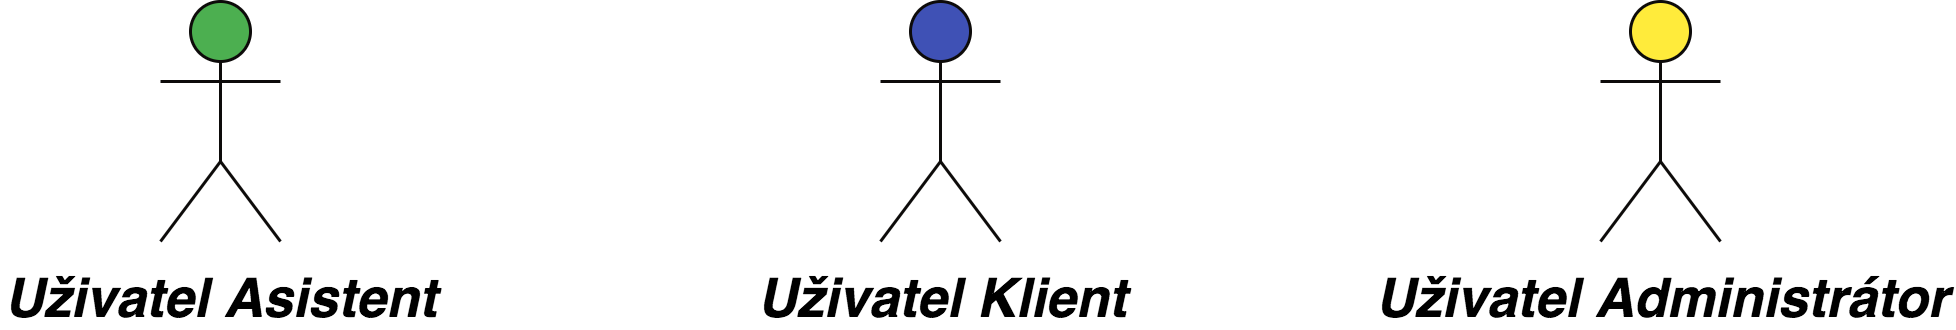
\includegraphics[scale=0.14]{img/actors.png}
        \caption{Aktéři systému}
        \label{fig:actors}
\end{figure}

Pro uživatele klienta i asistenta jsou definovány případy užití zvlášť, neboť se celé chování
a použití aplikace bude v obou případech značně lišit. Grafické zobrazní aktéru je na obrázku~\ref{fig:actors}.

\subsubsection{Uživatel Asistent}
Jedná se o aktéra, který je zároveň klientovi s mentálním postižením odborným asistentem,
jenž o něj pečuje a poskytuje mu podporu. Tento aktér je relevantní k vytváření obsahu,
který má pomoci klientovi k lepší orientaci při cestování a také mu může připravenou
cestu předvést. Může také nahraná data editovat a případně je rozšiřovat. Může také zadat
do aplikace zadat své kontaktní údaje pro možnou nečekanou situaci klienta na cestách, případně
nastavit zálohování uložených dat pro zamezení jejich ztráty při ztrátě telefonu nebo jeho výměně
za jiný.

\subsubsection{Uživatel Klient}
Klient je osoba pro kterou je aplikace primárně určena a má mu pomoci vyřešit problém,
v tomto případě pomoci z orientací při cestování. Může si prohlížet obsah a zejména ho
využívat při cestách v terénu. Uživatel by měl být upozorněn na všechny uložené a rozeznané
data v závislosti na své pozici a měl by tak získat relevantní informace k tomu, kde se právě
nachází. Dále může aplikaci využít ke snadnému kontaktování svého asistenta.



\subsubsection{Uživatel Administrátor}


\subsection{Use casy uživatel Asistent}
Pro uživatele asistenta jsou určeny složitější operace pro vytváření interaktivního obsahu pro klienta,
nastavování aplikace a prezentace klientovi. Pro use casy asistenta platí, že klient může těmto
krokům přihlížet, pokud o to projeví zájem. Use casy asistenta a jejich vztahy lze vidět na obrázku~\ref{fig:UseCasesAsistant}.

\begin{figure}[H]
        \centering
                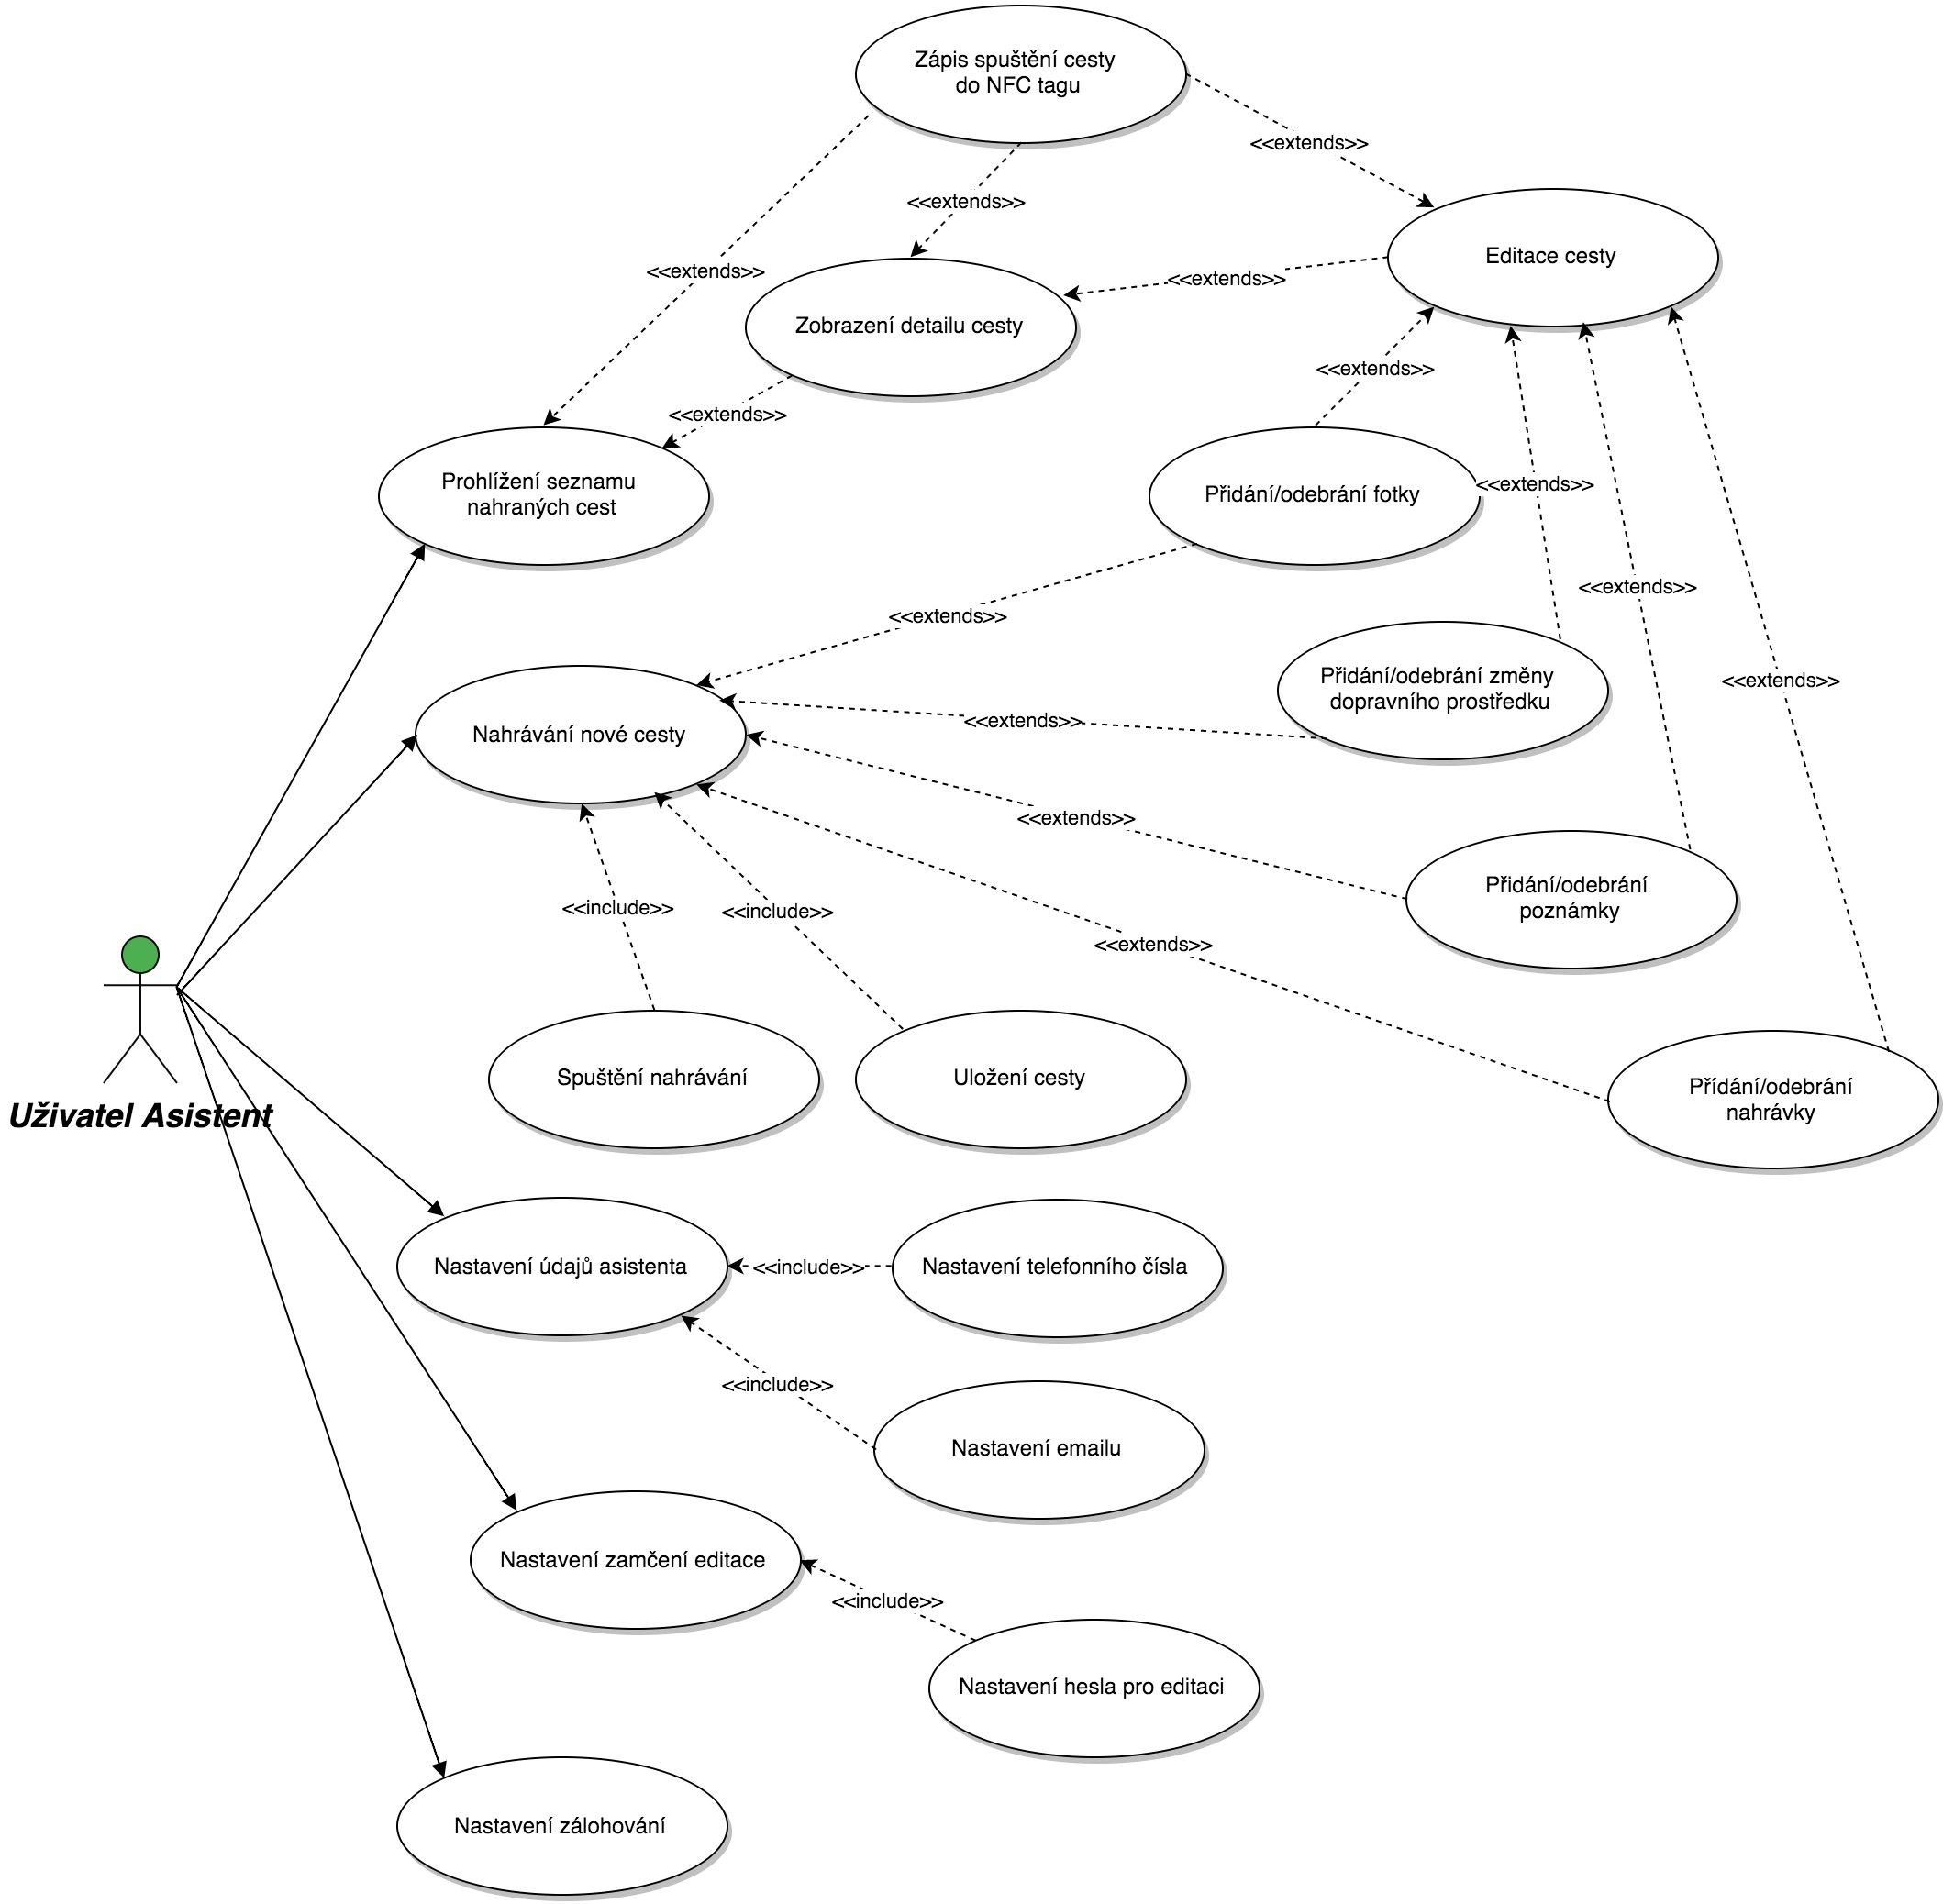
\includegraphics[scale=0.2]{img/UseCasesAsistant.png}
        \caption{Diagram use casů uživatele asistent}
        \label{fig:UseCasesAsistant}
\end{figure}

\usecase{Prohlížení seznamu nahraných cest}{prohlizeniasistent}
\textbf{Aktéři:} Asistent

\vspace{0.1cm}
\noindent
\textbf{Hlavní scénář:} Na úvodní obrazovce jsou zobrazeny všechny dosud nahrané cesty ve seznamu pod sebou.
Lze vidět pouze základní údaje a přiřazený obrázek pro snadnou orientaci. Uživatel se pomocí
kliknutí na řádek může podívat na celý detail cesty, případně pomocí rychlých akcí spustit ihned asistenci
a podobně. Obrazovku prohlížení cest lze vidět na obrázku~\ref{fig:prohlizeniasistent}.

\vspace{0.1cm}
\noindent
\textbf{Spouštěč:} Uživatel spustí aplikaci nebo se do ní vrátí pomocí notifikace v notifikační liště.

\vspace{0.1cm}
\noindent
\textbf{Rozšíření:}
\begin{itemize}
  \item \nameref{nahravanicesty}
  \item \nameref{detailasistent}
  \item \nameref{nfczapis}
\end{itemize}

\begin{figure}[H]
\begin{minipage}{.5\textwidth}
\centering
                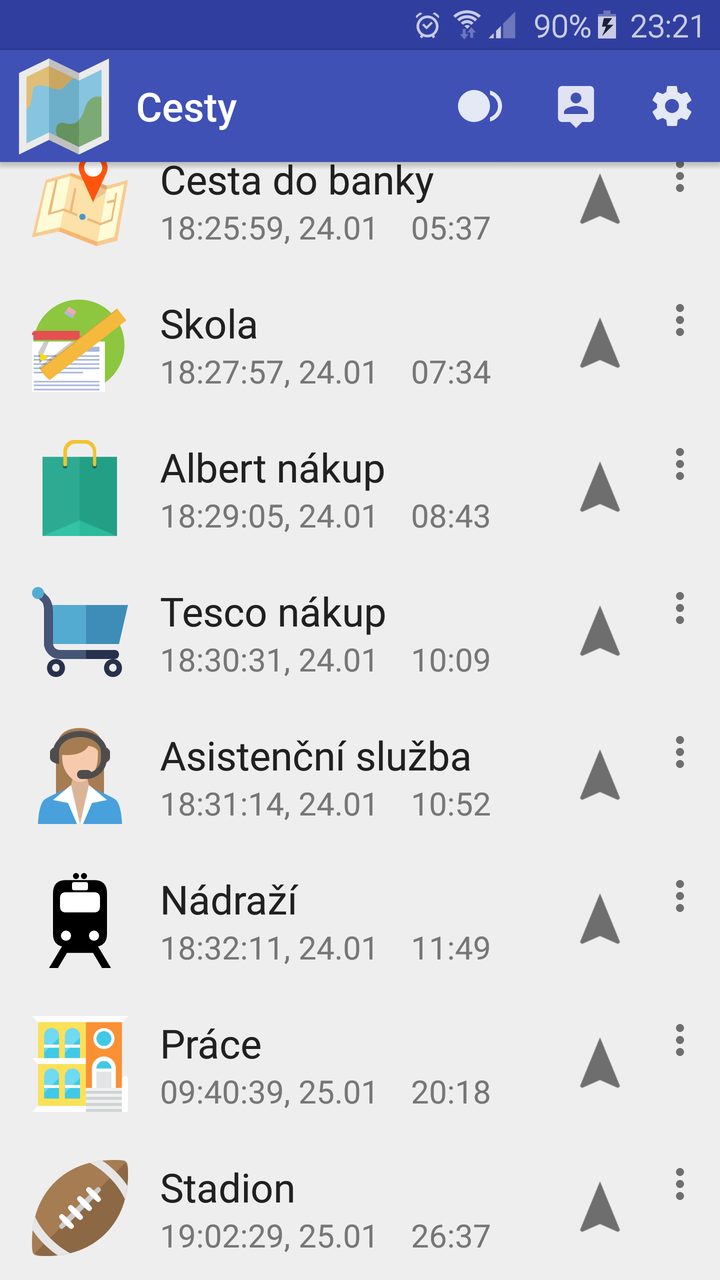
\includegraphics[scale=0.14]{img/screen/seznamcest.png}
        \caption{Prohlížení seznamu cest}
        \label{fig:prohlizeniasistent}
\end{minipage}
\begin{minipage}{.5\textwidth}
    \centering
                    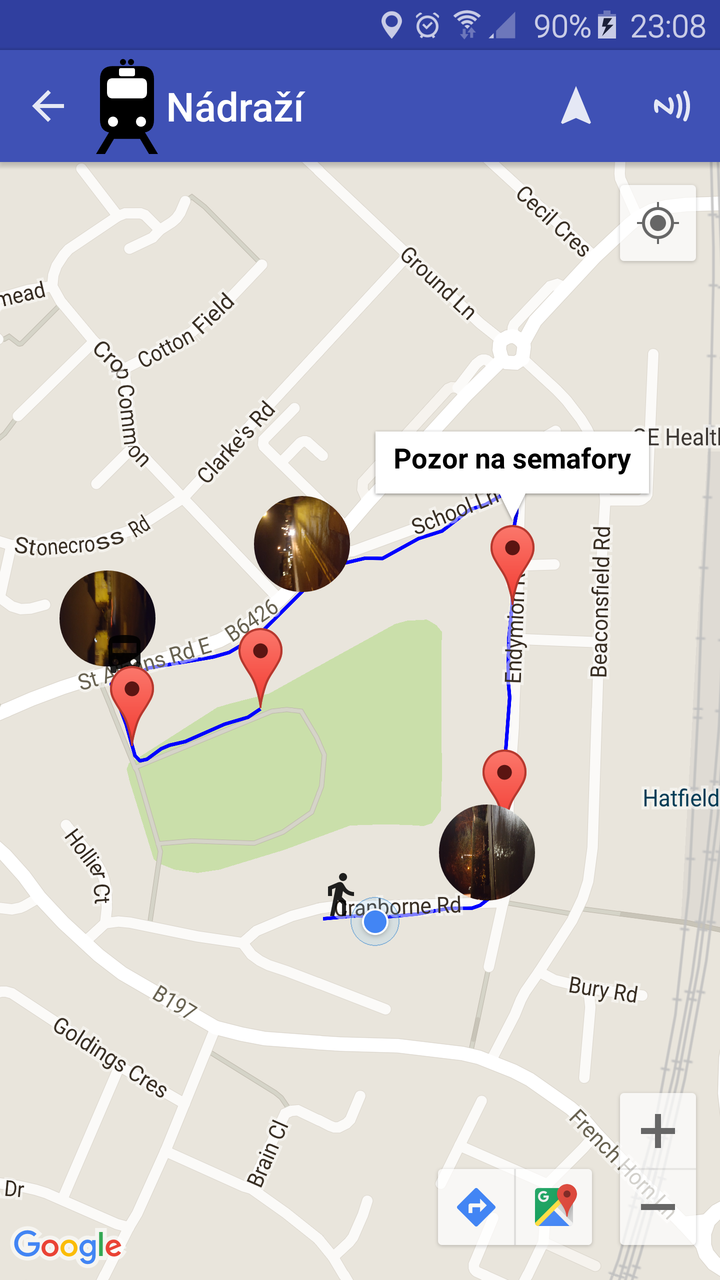
\includegraphics[scale=0.14]{img/screen/detailcesty.png}
            \caption{Zobrazení detailu cesty}
            \label{fig:detailasistent}

       \end{minipage}
\end{figure}

\usecase{Zobrazení detailu cesty}{detailasistent}
\textbf{Aktéři:} Asistent

\vspace{0.1cm}
\noindent
\textbf{Hlavní scénář:} Uživateli se zobrazí detail cesty se všemi informacemi, které jsou o ní uloženy.
Na mapě si může prohlédnout kudy vedla, an místech fotografií jsou miniatury fotek, při změně dopravních
prostředků lze vidět ikony daných prostředků, zvukově a textové záznamy jsou označeny příslušnou ikonou.
Při klepnutí na indikátor některého z těchto záznamů se zobrazí jeho popis, který uživatel dříve zadal.
V detailu cesty lze poklepáním na tlačítko editovat přejít do módu editace cesty a všechny dříve zmíněné
záznamy upravit. Ukázku lze vidět na obrázku~\ref{fig:detailasistent}.

\vspace{0.1cm}
\noindent
\textbf{Prekondice:} Cesta je uložena.

\vspace{0.1cm}
\noindent
\textbf{Spouštěč:} Uživatel klepne na řádek se zobrazenou cestou v seznamu cest.

\vspace{0.1cm}
\noindent
\textbf{Rozšíření:}
\begin{itemize}
  \item \nameref{editacecesty}
  \item \nameref{nfczapis}
\end{itemize}






\usecase{Zapsání cesty do NFC tagu}{nfczapis}
\textbf{Aktéři:} Asistent

\vspace{0.1cm}
\noindent
\textbf{Hlavní scénář:} Uživateli se zobrazí
obrazovka, která jej instruuje k přiložení NFC tagu k telefonu. Jakmile telefon zaznamená blízkost tagu,
zapíše do něj informaci o uložené cestě pro následné rychlé spouštění při přiložení tagu k telefonu.
Obrazovku zápisu do NFC tagu lze vidět na obrázku~\ref{fig:nfczapis} a oznámení o zapsaném tagu
na obrázku~\ref{fig:nfczapsano}.

\vspace{0.1cm}
\noindent
\textbf{Prekondice:} Cesta je uložena.

\vspace{0.1cm}
\noindent
\textbf{Spouštěč:} Uživatel klepne na ikonu NFC v detailu cesty nebo an rozšiřující menu v seznamu cest.


\begin{figure}[H]
\begin{minipage}{.5\textwidth}
\centering
                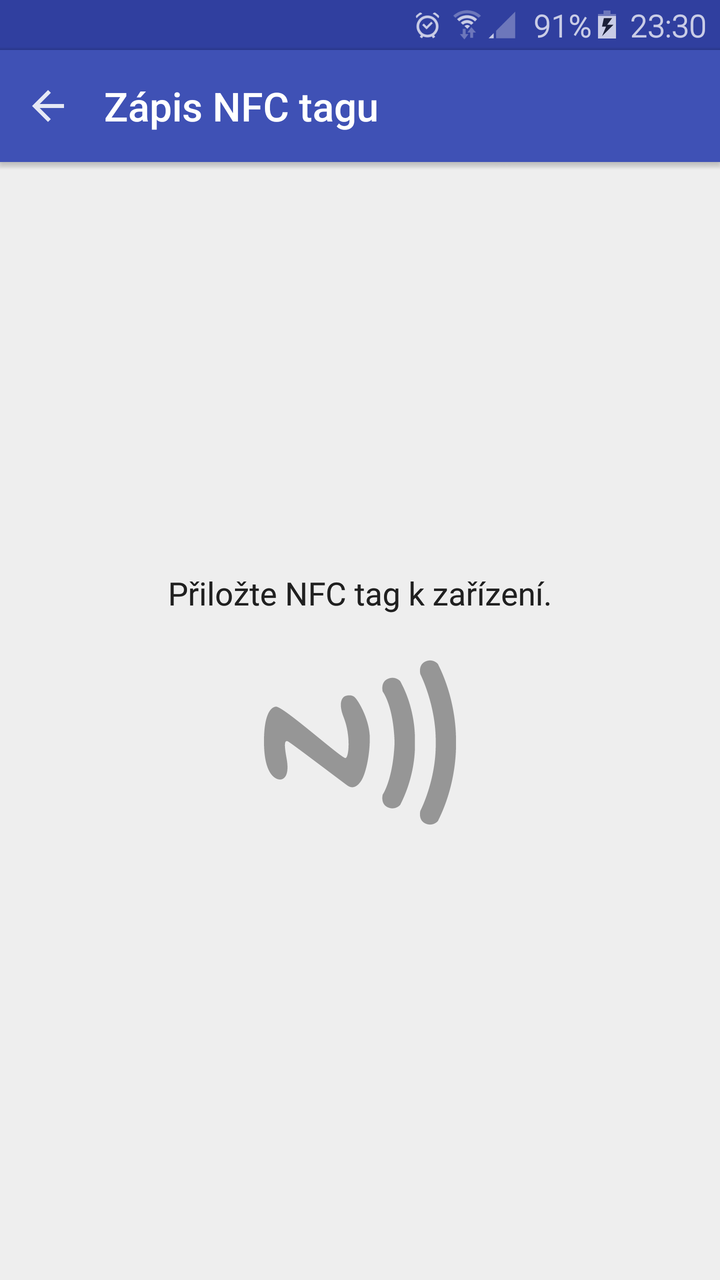
\includegraphics[scale=0.14]{img/screen/zapisnfcdetail.png}
        \caption{Zápis do NFC tagu}
        \label{fig:nfczapis}
\end{minipage}
\begin{minipage}{.5\textwidth}
    \centering
                    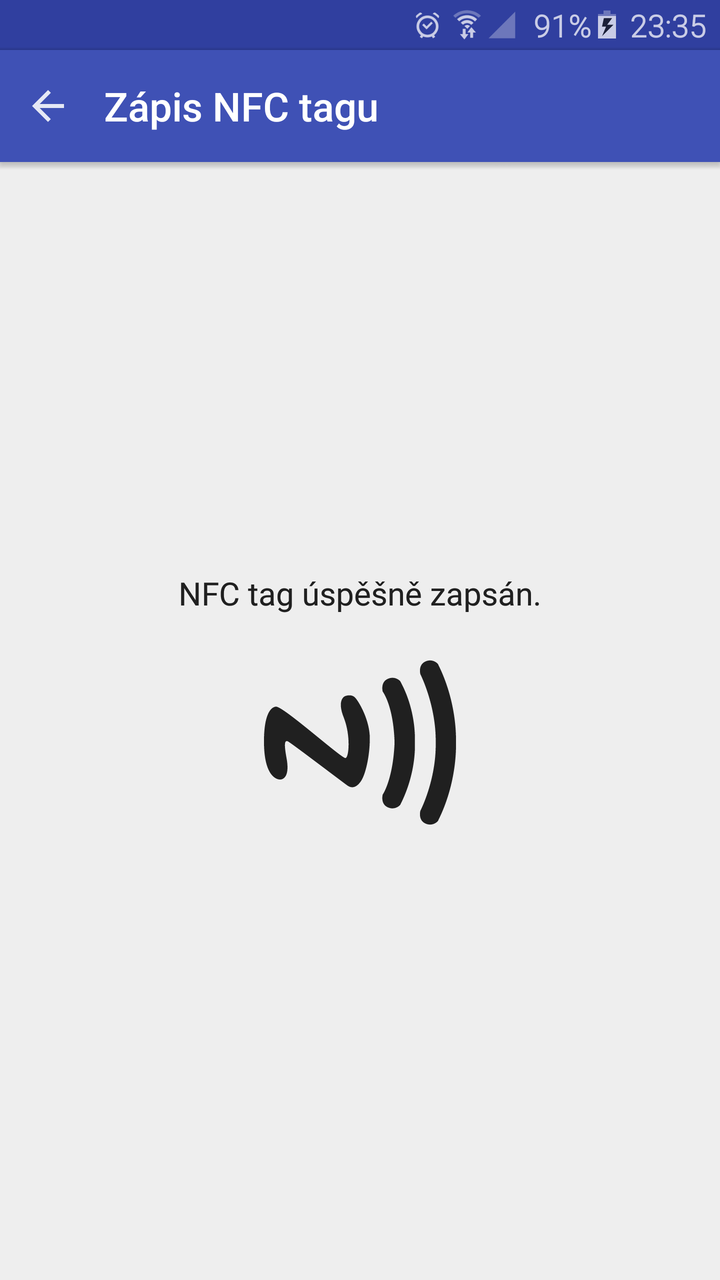
\includegraphics[scale=0.14]{img/screen/zapisdonfc.png}
            \caption{Zapsáno do NFC tagu}
            \label{fig:nfczapsano}

       \end{minipage}
\end{figure}



\usecase{Editace cesty}{editacecesty}
\textbf{Aktéři:} Asistent

\vspace{0.1cm}
\noindent
\textbf{Hlavní scénář:} Uživatel může editovat všechny uložené informace o cestě. Přepsání editačních
polí může změnit názvy a popis nahrané cesty, podržením a přetažením miniatur fotek nebo ikon dalších údajů na mapě může změnit
jejich pozici a tudíž místo, kdy se později vyvolají. Dále může podržením přetažením měnit tvar trasy,
při klepnutí na mapu přidat další záznamy. Jakmile je uživatel s editací spokojen, klepnutím na tlačítko
uložit se údaje zapíší do databáze a následující asistence cestování bude tyto údaje používat.

\vspace{0.1cm}
\noindent
\textbf{Prekondice:} Cesta je uložena.

\vspace{0.1cm}
\noindent
\textbf{Spouštěč:} Uživatel klepne na tlačítko editovat v detailu cesty.

\vspace{0.1cm}
\noindent
\textbf{Rozšíření:}
\begin{itemize}
  \item \nameref{pridanifotky}
  \item \nameref{pridaninahravky}
  \item \nameref{pridanipoznamky}
  \item \nameref{pridanizmenyprostredku}
    \item \nameref{odebranifotky}
    \item \nameref{odebraninahravky}
    \item \nameref{odebranipoznamky}
    \item \nameref{odebranizmenyprostredku}
\end{itemize}

\usecase{Přidání fotky}{pridanifotky}
\textbf{Aktéři:} Asistent

\vspace{0.1cm}
\noindent
\textbf{Hlavní scénář:} Spustí se fotoaparát zařízení a uživatel může začít fotit. Jakmile pořídí
fotografii, zobrazí se v aplikace okno pro zadání názvu fotky s dotazem pro uložení. Uživatel zadá název
a klepnutím na potvrzovací tlačítko se fotka uloží mezi data aplikace a zobrazí mezi aktuálními fotografiemi
na místě polohy uživatele v době pořízení fotografie. Uložení fotky lze vidět na obrázku~\ref{fig:pridanifotky}.

\vspace{0.1cm}
\noindent
\textbf{Prekondice:} Uživatel nahrává nebo edituje cestu.

\vspace{0.1cm}
\noindent
\textbf{Spouštěč:} Uživatel klepl na tlačítko přidat fotku.

\begin{figure}[H]
\begin{minipage}{.5\textwidth}
\centering
                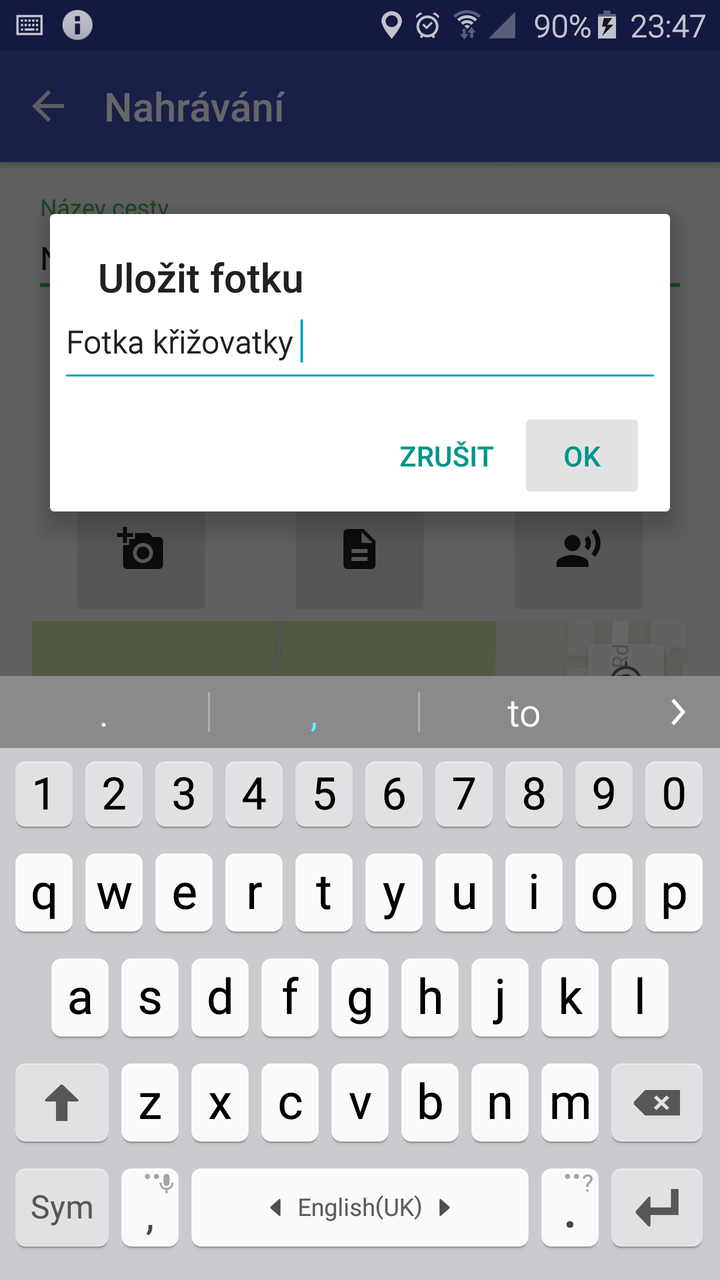
\includegraphics[scale=0.14]{img/screen/ulozenifotky.png}
        \caption{Pojmenování fotky po pořízení}
        \label{fig:pridanifotky}
\end{minipage}
\begin{minipage}{.5\textwidth}
     \centering
                     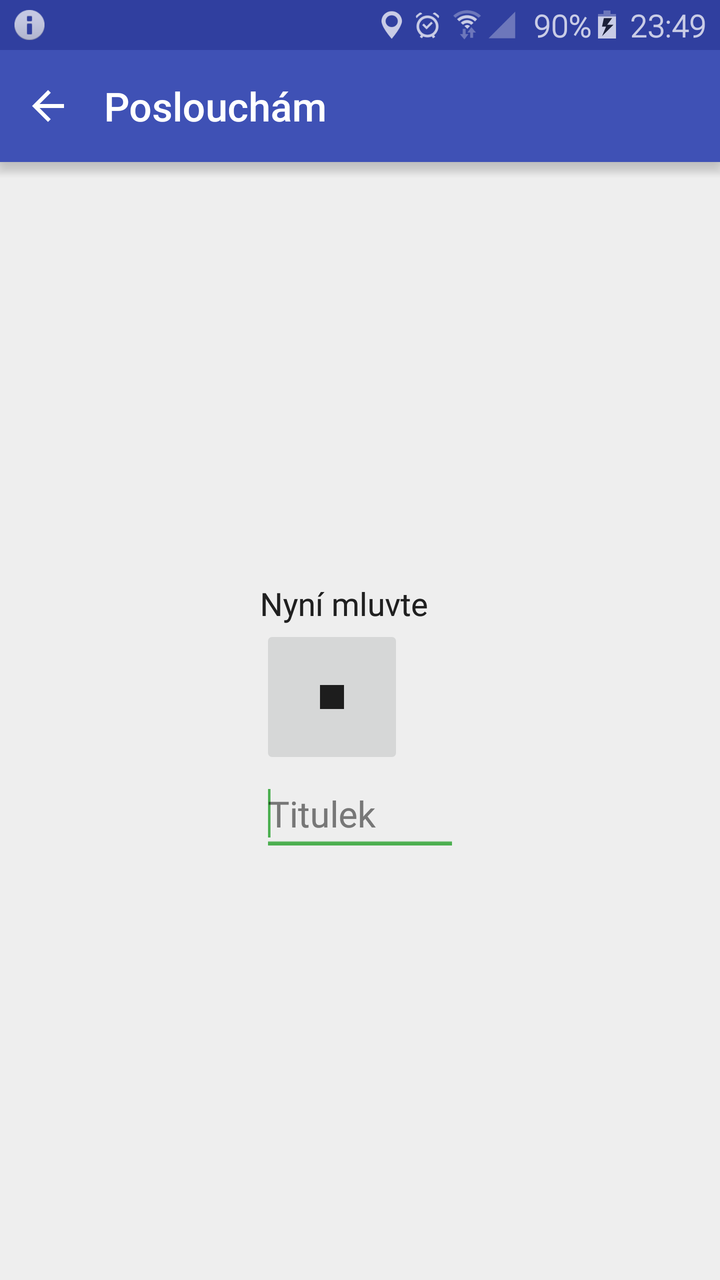
\includegraphics[scale=0.14]{img/screen/nahravaninahravky.png}
             \caption{Přidání zvukové nahrávky}
             \label{fig:pridaninahravky}

       \end{minipage}
\end{figure}

\usecase{Přidání zvukové nahrávky}{pridaninahravky}
\textbf{Aktéři:} Asistent

\vspace{0.1cm}
\noindent
\textbf{Hlavní scénář:} Uživateli se zobrazí obrazovka s textem mluvte a zvuk se zaznamenává.
Když je uživatel hotov, klepne na tlačítko stop a může nahrávce přidat název, který se bude později zobrazovat.
Poté tlačítkem nahrávku uloží mezi data aplikace s přiřazenou aktuální polohou uživatele.
Zobrazení nahrávání lze vidět na obrázku~\ref{fig:pridaninahravky}.

\vspace{0.1cm}
\noindent
\textbf{Prekondice:} Uživatel nahrává nebo edituje cestu.

\vspace{0.1cm}
\noindent
\textbf{Spouštěč:} Uživatel klepl na tlačítko přidat nahrávku.




\usecase{Přidání poznámky}{pridanipoznamky}
\textbf{Aktéři:} Asistent

\vspace{0.1cm}
\noindent
\textbf{Hlavní scénář:} Uživateli se zobrazí okno s textovým vstupem a vysune se klávesnice. Uživatel
zadá textovou poznámku a po klepnutí na potvrzovací tlačítko se poznámka uloží s asociací k aktuální poloze
uživatele. Okno přidávání poznámky lze vidět na obrázku~\ref{fig:pridanipoznamky}.

\vspace{0.1cm}
\noindent
\textbf{Prekondice:} Uživatel nahrává nebo edituje cestu.

\vspace{0.1cm}
\noindent
\textbf{Spouštěč:} Uživatel klepl na tlačítko přidat poznámku.

\begin{figure}[H]
\begin{minipage}{.5\textwidth}
\centering
                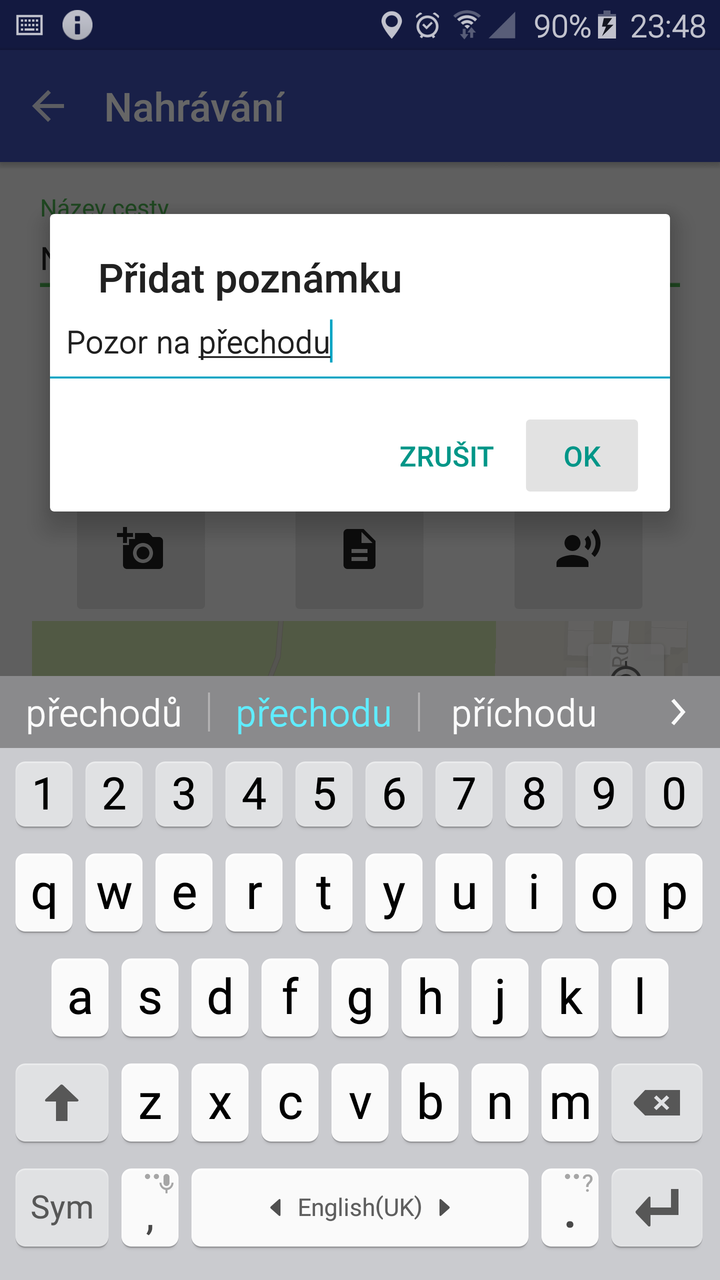
\includegraphics[scale=0.14]{img/screen/pridanipoznamky.png}
        \caption{Přidání poznámky}
        \label{fig:pridanipoznamky}
\end{minipage}
\begin{minipage}{.5\textwidth}
  \centering
                  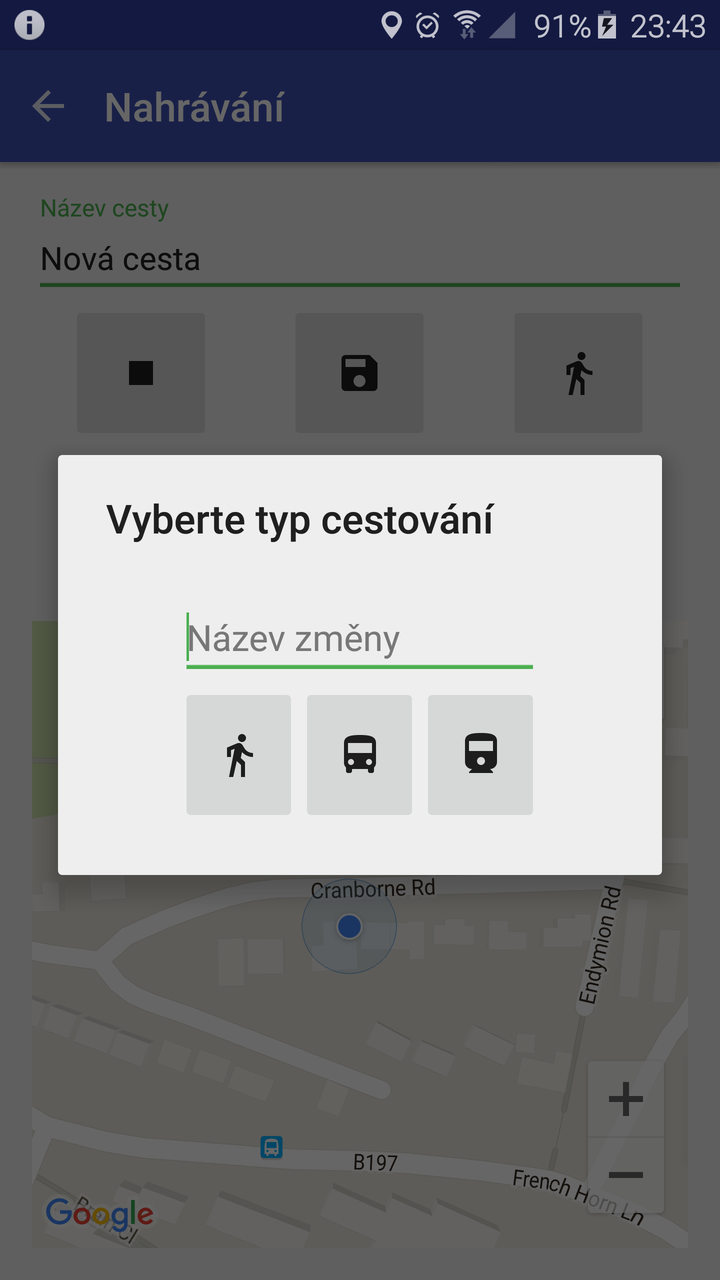
\includegraphics[scale=0.14]{img/screen/zmenaprostredku.png}
          \caption{Změna dopravního prostředku}
          \label{fig:pridanizmenyprostredku}

       \end{minipage}
\end{figure}

\usecase{Přidání změny dopravního prostředku}{pridanizmenyprostredku}
\textbf{Aktéři:} Asistent


\vspace{0.1cm}
\noindent
\textbf{Hlavní scénář:} Zobrazí se okno se nabídkou tlačítek s obrázkem dopravního prostředku.
Uživatel může zároveň přidat ke změně dopravního prostředku přidat popis. Po kliknutí na
tlačítko s dopravním prostředkem se změna dopravního prostředku uloží s asociovanou aktuální polohou
uživatele. Okno změny dopravního prostředku lze vidět na obrázku~\ref{fig:pridanizmenyprostredku}.

\vspace{0.1cm}
\noindent
\textbf{Prekondice:} Uživatel nahrává nebo edituje cestu.

\vspace{0.1cm}
\noindent
\textbf{Spouštěč:} Uživatel klepl na tlačítko s aktuálním dopravním prostředkem.




\usecase{Nahrávání cesty}{nahravanicesty}
\textbf{Aktéři:} Asistent

\vspace{0.1cm}
\noindent
\textbf{Hlavní scénář:} Uživateli se zobrazí nahrávací okno, kde může vidět svou aktuální pozici
a po klepnutí na tlačítko nahrávat začne aplikace sbírat data o poloze a umožní mu přidávat další data
k právě nahrávané pozici. V notifikační liště se objeví notifikace o tom, že aplikace právě nahrává.
Uživatel může v tu chvíli odejít z aplikace, případně navštívit její jiné obrazovky a poté se do nahrávání vrátit,
aniž by ztratil právě nahrávaná data. Stejně tak po opuštění aplikace při nahrávání se do ní může vrátit
klepnutím na zobrazenou notifikaci.

Na mapě vidí uživatel dosud nahranou a uloženou cestu a případné přidané data.
Klepnutím na tlačítko uložit se aktuálně nahraní data a média uloží, případně aktualizují.
Pokud uživatel dokončil nahrávání cesty, klepne na tlačítko uložit a poté tlačítkem stop zastaví nahrávání,
notifikace zmizí a cesta je v seznamu cest připraveno pro spuštění asistence, případně následnou editaci.
Pokud uživatel ukončí nahrávání bez uložení, je na toto upozorněn a při potvrzení ukončení jsou nahraná data
smazána. Obrazovku nahrávání můžeme vidět na obrázku~\ref{fig:nahravanicesty} a zobrazenou notifikaci
na obrázku~\ref{fig:notifikacenahravanicesty}.

\vspace{0.1cm}
\noindent
\textbf{Prekondice:} Uživatel má v telefonu povolené získávání polohy pomocí GPS.

\vspace{0.1cm}
\noindent
\textbf{Spouštěč:} Uživatel klepne na tlačítko nahrávat v seznamu nahraných cest.

\vspace{0.1cm}
\noindent
\textbf{Rozšíření:}
\begin{itemize}
  \item \nameref{pridanifotky}
  \item \nameref{pridaninahravky}
  \item \nameref{pridanipoznamky}
  \item \nameref{pridanizmenyprostredku}
  \item \nameref{odebranifotky}
  \item \nameref{odebraninahravky}
  \item \nameref{odebranipoznamky}
  \item \nameref{odebranizmenyprostredku}
\end{itemize}

\begin{figure}[H]
\begin{minipage}{.5\textwidth}


        \centering
                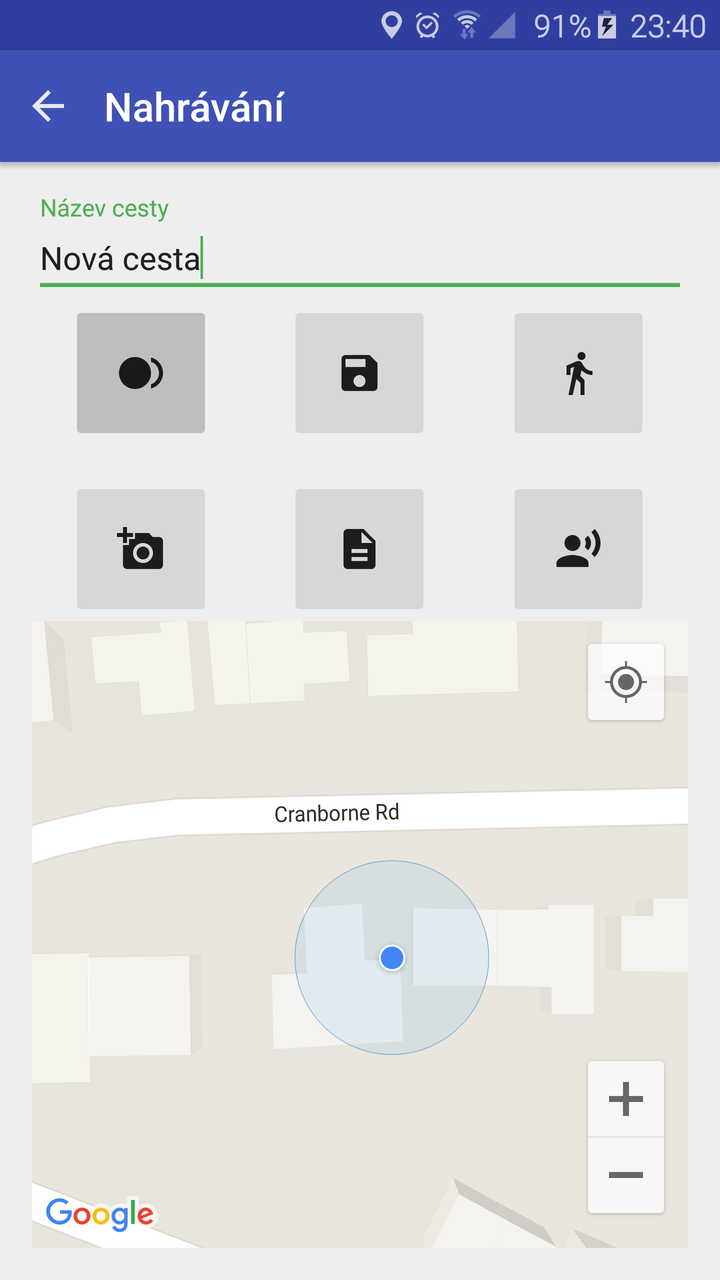
\includegraphics[scale=0.14]{img/screen/nahravani.png}
        \caption{Nahrávání cesty}
        \label{fig:nahravanicesty}
\end{minipage}
\begin{minipage}{.5\textwidth}
  \centering
                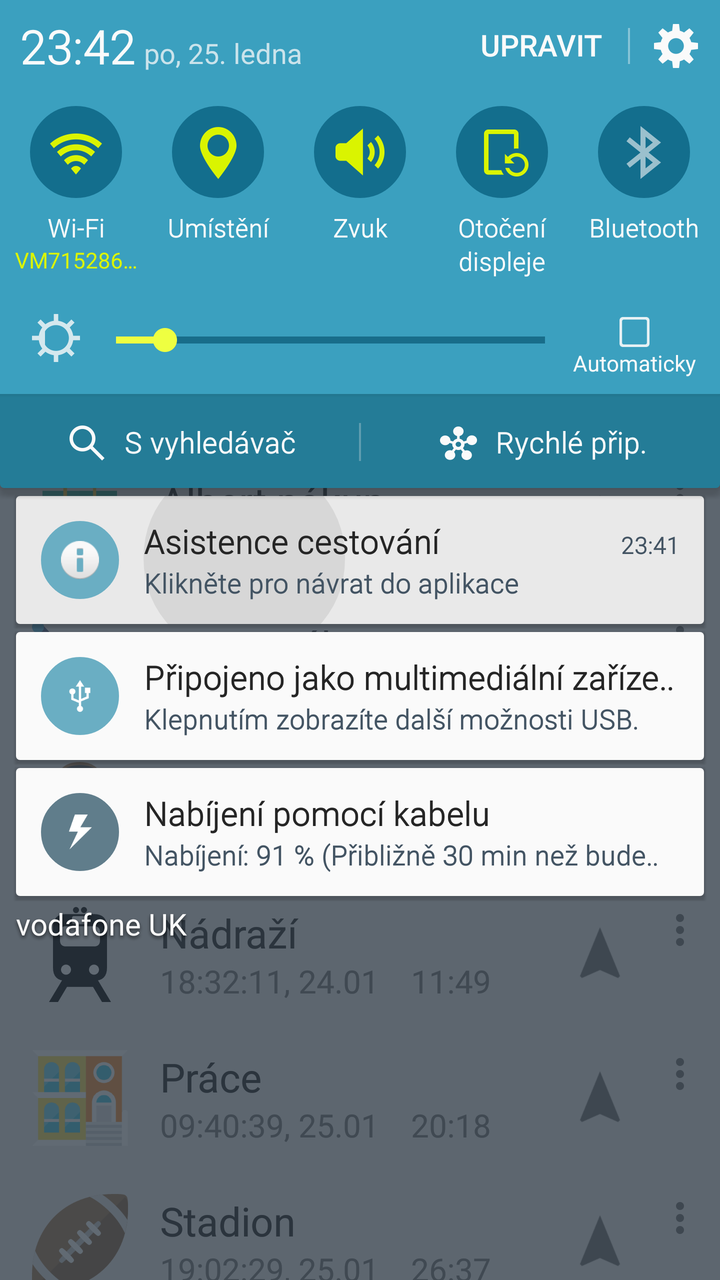
\includegraphics[scale=0.14]{img/screen/notifikace.png}
        \caption{Zobrazená notifikace}
        \label{fig:notifikacenahravanicesty}

       \end{minipage}
\end{figure}


\usecase{Odebrání fotky}{odebranifotky}
\textbf{Aktéři:} Asistent

\vspace{0.1cm}
\noindent
\textbf{Hlavní scénář:} Uživateli se zobrazí okno s dotazem zda chce fotku odebrat. Po klepnutí na
potvrzovací tlačítko je fotka smazána z úložiště a odstraněna její miniatura z aktuální cesty.

\vspace{0.1cm}
\noindent
\textbf{Prekondice:} Uživatel nahrává nebo edituje cestu a má uloženou fotografii.

\vspace{0.1cm}
\noindent
\textbf{Spouštěč:} Uživatel podrží prst na miniatuře fotografie a vybere možnost smazat.



\usecase{Odebrání zvukové nahrávky}{odebraninahravky}
\textbf{Aktéři:} Asistent

\vspace{0.1cm}
\noindent
\textbf{Hlavní scénář:} Uživateli se zobrazí dotaz zda chce nahrávku opravdu smazat, po potvrzení
se uložená nahrávka odstraní a zmizí její ikona.

\vspace{0.1cm}
\noindent
\textbf{Prekondice:} Uživatel nahrává nebo edituje cestu a má uloženou nahrávku.

\vspace{0.1cm}
\noindent
\textbf{Spouštěč:} Uživatel podrží prst na ikoně nahrávky a vybere možnost smazat.



\usecase{Odebrání poznámky}{odebranipoznamky}
\textbf{Aktéři:} Asistent

\vspace{0.1cm}
\noindent
\textbf{Hlavní scénář:} Uživateli se zobrazí okno s dotazem na smazání poznámky. Po potvrzení se
nahrávka smaže a zmizí ikona indikující nahrávku.

\vspace{0.1cm}
\noindent
\textbf{Prekondice:} Uživatel nahrává nebo edituje cestu a má uloženou poznámku.

\vspace{0.1cm}
\noindent
\textbf{Spouštěč:} Uživatel podrží prst na ikoně poznámky a vybere možnost smazat.


\usecase{Odebrání změny dopravního prostředku}{odebranizmenyprostredku}
\textbf{Aktéři:} Asistent

\vspace{0.1cm}
\noindent
\textbf{Hlavní scénář:} Uživateli se zobrazí okno s dotazem na smazání změny dopravního prostředku.
Po potvrzení se nahrávka smaže a zmizí ikona indikující nahrávku. Zobrazené nstavení údajů
lze vidět na obrázku~\ref{fig:nastaveniudaju}.

\vspace{0.1cm}
\noindent
\textbf{Prekondice:} Uživatel nahrává nebo edituje cestu a má uloženou změnu dopravního prostředku.

\vspace{0.1cm}
\noindent
\textbf{Spouštěč:} Uživatel podrží prst na ikoně změny dopravního prostředku a vybere možnost smazat.


\usecase{Nastavení údajů asistenta}{nastaveniudaju}
\textbf{Aktéři:} Asistent

\vspace{0.1cm}
\noindent
\textbf{Hlavní scénář:} Uživateli se zobrazí obrazovka s nastavením údajů, kde může vyplnit své údaje.

\vspace{0.1cm}
\noindent
\textbf{Spouštěč:} Uživatel klepl na tlačítko nastavení.

\vspace{0.1cm}
\noindent
\textbf{Rozšíření:}
\begin{itemize}
  \item \nameref{nastavenicisla}
  \item \nameref{nastaveniemailu}
\end{itemize}

\begin{figure}[H]
\begin{minipage}{.5\textwidth}
\centering
                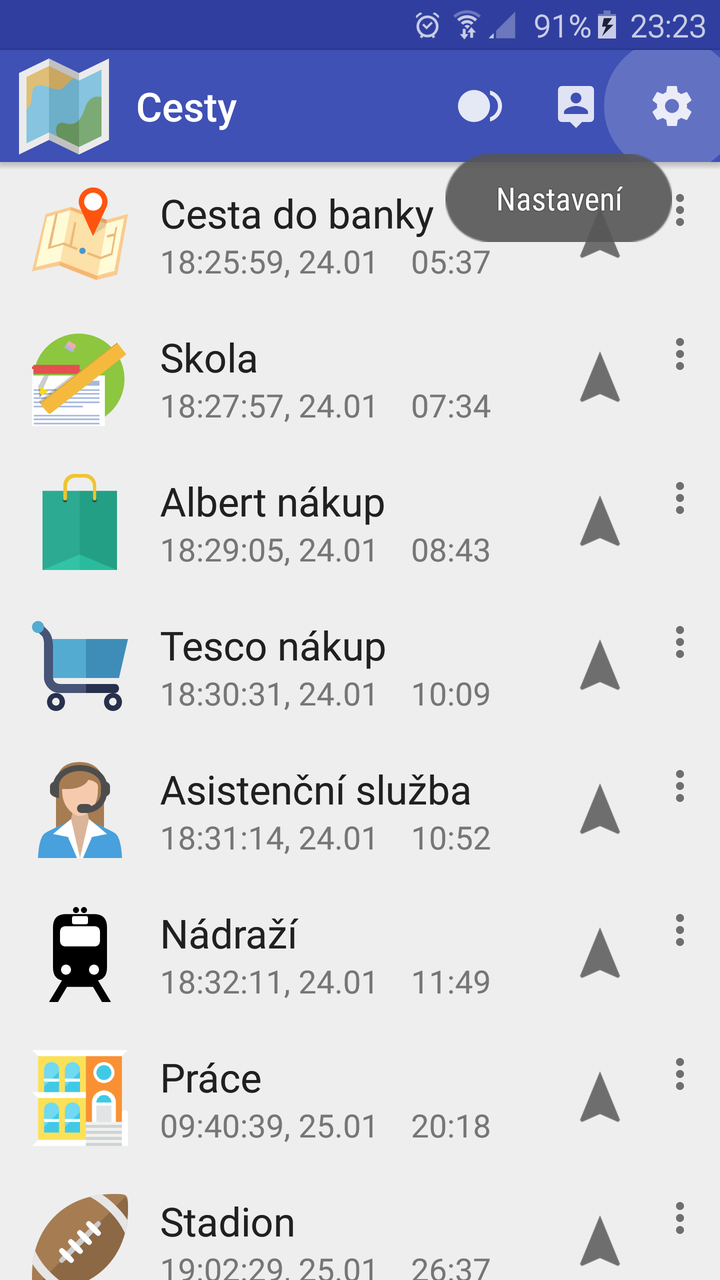
\includegraphics[scale=0.14]{img/screen/nastaveni.png}
        \caption{Spuštění nastavení údajů}
        \label{fig:nastaveniudaju}
\end{minipage}
\begin{minipage}{.5\textwidth}
\centering
                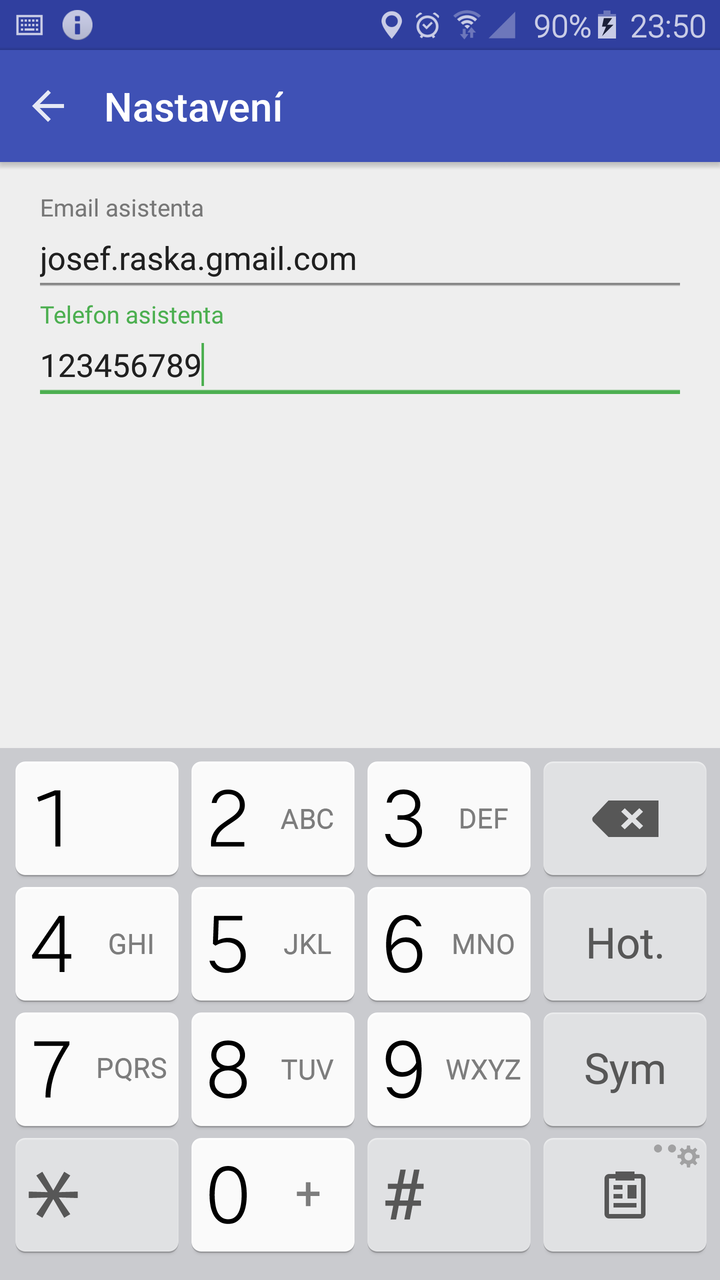
\includegraphics[scale=0.14]{img/screen/nastaveniasistent.png}
        \caption{Nastavení telefonního čísla}
        \label{fig:nastavenicisla}
    \end{minipage}
\end{figure}

\usecase{Nastavení telefonního čísla asistenta}{nastavenicisla}
\textbf{Aktéři:} Asistent

\vspace{0.1cm}
\noindent
\textbf{Hlavní scénář:} Editovatelné pole pro telefonní číslo se zvýrazní a vysune se numerická klávesnice.
Uživatel zadá své telefonní číslo, které se automaticky formátuje do přívětivějšího formátu. Po ukončení
editace je telefonní číslo automaticky uloženo. Pokud telefonní číslo neodpovídá formátu telefonních čísel
v České Republice, uživatel je na toto upozorněn a je vyzván k úpravě vstupu. Zadávání telefonního čísla
vidíme na obrázku~\ref{fig:nastavenicisla}.

\vspace{0.1cm}
\noindent
\textbf{Spouštěč:} Uživatel klepl na editační pole s telefonním číslem asistenta.

\usecase{Nastavení emailu asistenta}{nastaveniemailu}
\textbf{Aktéři:} Asistent

\vspace{0.1cm}
\noindent
\textbf{Hlavní scénář:} Editovatelné pole pro emailovou adresu se zvýrazní a vysune se klávesnice.
Uživatel zadá svou emailovou adresu. Po ukončení editace je emailová adresa automaticky uložena.
Pokud emailová adresa neodpovídá správnému formátu emailové adresy, uživatel je na toto upozorněn
a vyzván k úpravě vstupu.

\vspace{0.1cm}
\noindent
\textbf{Spouštěč:} Uživatel klepl na editovatelné pole emailové adresy.


\usecase{Nastavení zamčení editace}{nastavenizamceni}
\textbf{Aktéři:} Asistent

\vspace{0.1cm}
\noindent
\textbf{Hlavní scénář:} Uživateli se zobrazí editovatelné pole, kde může zadat heslo pro zamčení editace
obsahu aplikace. Pokud toto heslo nezadá, aplikace bude stále v módu editace a uložená data bude možné upravit.
Uživatel zadá heslo, to bude uloženo a bude nyní vyžadováno pro zpřístupnění úprav cest, případně nastavení.

\vspace{0.1cm}
\noindent
\textbf{Spouštěč:} Uživatel klepl na tlačítko nastavení zamčení.

\usecase{Nastavení zálohování}{nastavenizalohovani}
\textbf{Aktéři:} Asistent

\vspace{0.1cm}
\noindent
\textbf{Hlavní scénář:} Uživateli se zobrazí výběr z listu zda chce zálohovat manuálně, jednou za den, týden
nebo za měsíc. Uživatel vybere jednu z možností a podle výběru se naplánují příslušné akce.

\vspace{0.1cm}
\noindent
\textbf{Prekondice:} Uživatel má na zařízení uložen nastaven účet umožňující zálohování.

\vspace{0.1cm}
\noindent
\textbf{Spouštěč:} Uživatel klepl na tlačítko nastavení zálohování.


















\subsection{Use casy uživatele Klient}
Pro klienta jsou určeny více intuitivní a nenáročné operace vyžadující co nejméně aktivních
kroků z klientovi strany. Aplikace by měla na základě polohy a dalších údajů sama rozpoznat,
co má v danou chvíli udělat. Use casy klienta a jejich vztahy lze vidět na obrázku~\ref{fig:UseCasesClient}.

\begin{figure}[H]
        \centering
                \includegraphics[scale=0.2]{img/UseCasesClient.png}
        \caption{Diagram use casů uživatele klient}
        \label{fig:UseCasesClient}
\end{figure}


\usecase{Prohlížení seznamu nahraných cest}{prohlizeniklient}
\textbf{Aktéři:} Klient

\vspace{0.1cm}
\noindent
\textbf{Hlavní scénář:} Na úvodní obrazovce jsou pod sebou vyobrazeny všechny cesty, pro které může
uživateli aplikace poskytnout asistenci. Uživatel si prohlíží cesty, které mají zobrazeny pouze
základní informace a jsou označeny vybraným obrázkem pro snažší orientaci. Uživatel si poklepnutím
na řádek cesty může dostat na její detail případně rychlými akcemi spustí navigaci.

\vspace{0.1cm}
\noindent
\textbf{Spouštěč:} Uživatel klepne na ikonu aplikace v telefonu.

\vspace{0.1cm}
\noindent
\textbf{Rozšíření:}
\begin{itemize}
  \item \nameref{detailklient}
  \item \nameref{asistence}
\end{itemize}

\usecase{Detail nahrané cesty}{detailklient}
\textbf{Aktéři:} Klient

\vspace{0.1cm}
\noindent
\textbf{Hlavní scénář:} Klientovi se zobrazí obrazovka se všemi údaji, které mu mají na cestě pomoci.
Fotky jsou vidět jako miniatury na místě, kde byly pořízeny, podobně nahrávky, změny dopravního prostředku
a poznámky, které jsou reprezentovány svými příslušnými jednoduchými ikonami.

\vspace{0.1cm}
\noindent
\textbf{Prekondice:} Uživatel má nahranou cestu.

\vspace{0.1cm}
\noindent
\textbf{Spouštěč:} Uživatel klepne na řádek cesty v seznamu nahraných cest.

\vspace{0.1cm}
\noindent
\textbf{Rozšíření:}
\begin{itemize}
  \item \nameref{asistence}
\end{itemize}


\usecase{Asistence cestování}{asistence}
\textbf{Aktéři:} Klient

\vspace{0.1cm}
\noindent
\textbf{Hlavní scénář:} Uživateli se zobrazí jednoduchá mapka s vyznačenou cestou, kterou má absolvovat.
Zobrazí se mu všechny dostupné informace jako čas do cíle, doporučený směr, nejbližší nahrané fotky,
nahrávky nebo poznámky. Zkontroluje se podle uložených statistik, zda bude uživateli stačit baterie
k absolvování cesty a pokud ne, bude na to upozorněn.
Aplikace využívá klientovu polohu pro zobrazení relevantních nahraných informací
a snaží se mu napovídat následující směr pomocí zobrazené šipky. Jak se klient pohybuje, aplikace mu
poskytuje nahraný obsah asistentem, který by mu měl pomoci v danou chvíli se lépe zorientovat.
Obrazovku asistence cestování lze vidět na obrázku~\ref{fig:asistence}.

\vspace{0.1cm}
\noindent
\textbf{Prekondice:} Klient má nahranou cestu a spustil asistenci cestování po této cestě.

\vspace{0.1cm}
\noindent
\textbf{Spouštěč:} Klient klepl na obrázek navigovat.

\vspace{0.1cm}
\noindent
\textbf{Rozšíření:}
\begin{itemize}
  \item \nameref{zobrazenifotky}
  \item \nameref{prehraninahravky}
  \item \nameref{zobrazenipoznamky}
  \item \nameref{upozorneniprostredek}
  \item \nameref{analyzabaterie}
  \item \nameref{zobrazenismeru}
  \item \nameref{upozorneninespravnysmer}
\end{itemize}


\begin{figure}[H]
\begin{minipage}{.5\textwidth}
\centering
                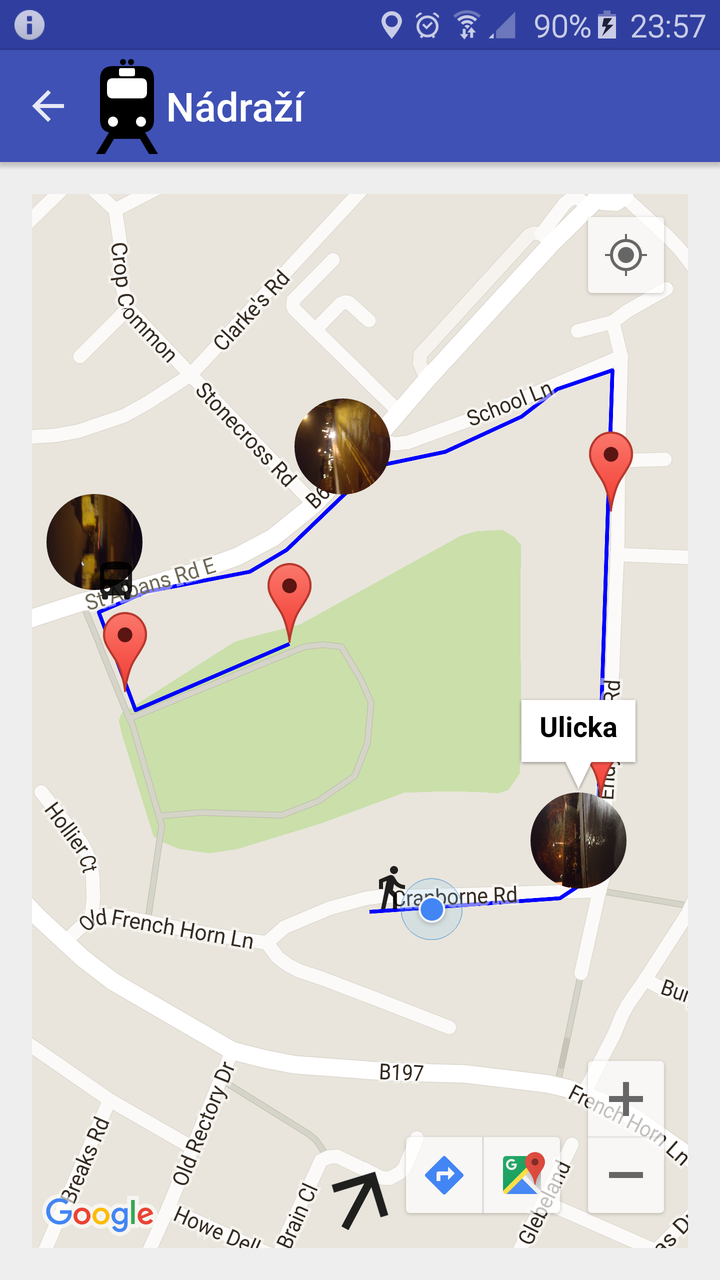
\includegraphics[scale=0.14]{img/screen/asistencecestovani.png}
        \caption{Asistence cestování}
        \label{fig:asistence}
\end{minipage}
\begin{minipage}{.5\textwidth}
\centering
                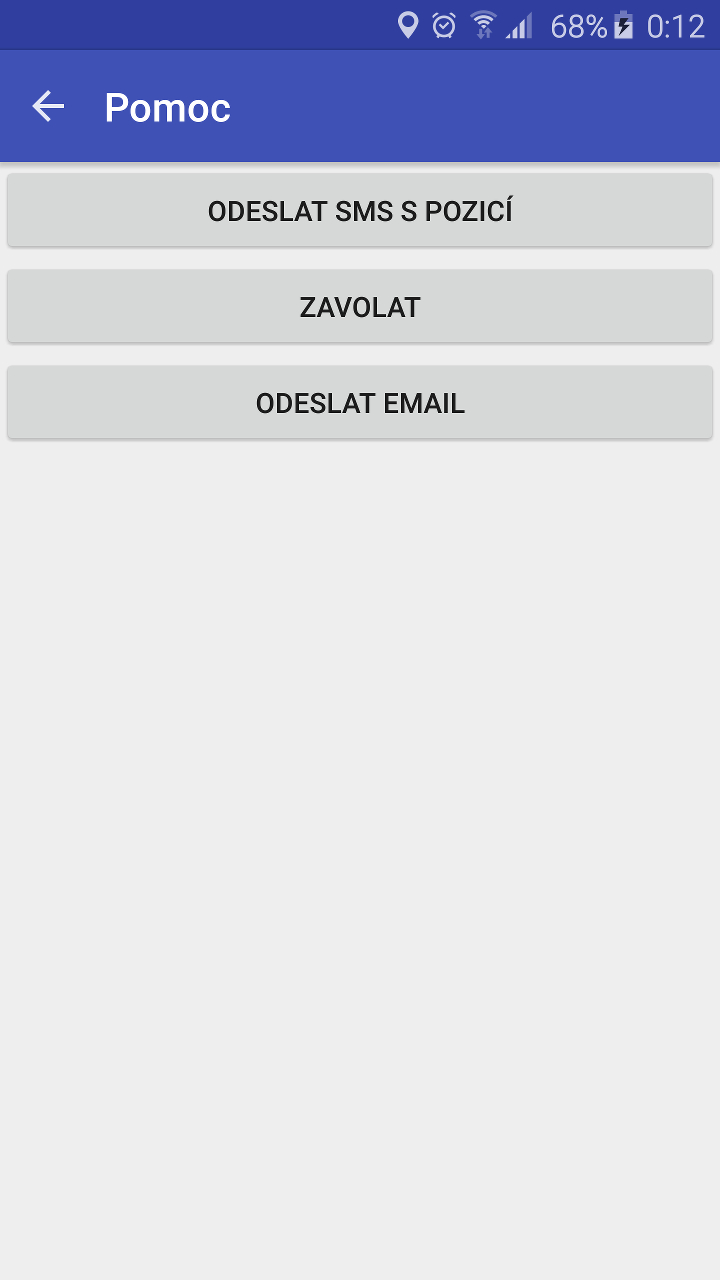
\includegraphics[scale=0.14]{img/screen/volanipomoc.jpg}
        \caption{Obrazovka pomoci}
        \label{fig:pomoc}
    \end{minipage}
\end{figure}



\usecase{Zobrazení fotografie}{zobrazenifotky}
\textbf{Aktéři:} Klient

\vspace{0.1cm}
\noindent
\textbf{Hlavní scénář:} Uživatel se přiblíží k místu pořízení fotografie, aplikace toto rozpozná
a upozorní uživatele na přítomnost fotky, která se zobrazí na dobu, po kterou je uživatel nablízku.
Přes spodní část fotky je zobrazen popisek, který této fotce dříve zadal asistent.

\vspace{0.1cm}
\noindent
\textbf{Prekondice:} Uživatel má k dané cestě uloženou fotku.

\vspace{0.1cm}
\noindent
\textbf{Spouštěč:} Uživatel se přiblíží místu pořízení fotky nebo klepne na miniaturu fotky.


\usecase{Přehrání uložené zvukové nahrávky}{prehraninahravky}
\textbf{Aktéři:} Klient

\vspace{0.1cm}
\noindent
\textbf{Hlavní scénář:} Uživatel se se zapnutou asistencí cestování přiblíží místu,
kde byla dríve za pomoci asistenta pořízena zvuková nahrávka. Uložená nahrávka se načte
a začne se uživateli přehrávat. Zároveň se zobrazí popis nahrávky a tlačítko umožňující
nahrávku přehrát znovu.

\vspace{0.1cm}
\noindent
\textbf{Prekondice:} Uživatel má k dané cestě uloženou zvukovou nahrávku.

\vspace{0.1cm}
\noindent
\textbf{Spouštěč:} Uživatel se přiblíží k místu pořízení nahrávky nebo klepne na ikonu nahrávky.

\usecase{Zobrazení uložené poznámky}{zobrazenipoznamky}
\textbf{Aktéři:} Klient

\vspace{0.1cm}
\noindent
\textbf{Hlavní scénář:} Uživatel je při přiblížení se místu poznámky upozorněn a poznámka se zobrazí.

\vspace{0.1cm}
\noindent
\textbf{Prekondice:} Uživatel má k dané cestě uloženou poznámku.

\vspace{0.1cm}
\noindent
\textbf{Spouštěč:} Uživatel se přiblíží k místu pořízení poznámky nebo klepne na ikonu poznámky.

\usecase{Upozornění na změnu dopravního prostředku}{upozorneniprostredek}
\textbf{Aktéři:} Klient

\vspace{0.1cm}
\noindent
\textbf{Hlavní scénář:} Uživateli je při přiblížení ke změně dopravního prostředku upozorněn,
zobrazí se mu obrázek dopravního prostředku, do kterého má nastoupit nebo naopak vystoupit spolu
s textem, který byl při nahrávání cesty zadán.

\vspace{0.1cm}
\noindent
\textbf{Prekondice:} Uživatel má uloženo upozornění na změnu dopravního prostředku.

\vspace{0.1cm}
\noindent
\textbf{Spouštěč:} Uživatel se přiblíží k místu změny dopravního prostředku.



\usecase{Analýza spotřeby baterie}{analyzabaterie}
\textbf{Aktéři:} Klient

\vspace{0.1cm}
\noindent
\textbf{Hlavní scénář:} Během cestování se ukládají průběžně data o spotřebě beterie a délce trvání
cesty. Data jsou poté spolu s předchozími záznamy statisticky analyzována a je odhadována a upřesňována
očekávaná výdrž baterie během navigace. Na základě těchto analýz může být uživatel poté upozorněn na
nebezpečí vybití baterie v terénu.

\vspace{0.1cm}
\noindent
\textbf{Spouštěč:} Uživatel využívá asistence při cestování.



\usecase{Zobrazení doporučeného směru}{zobrazenismeru}
\textbf{Aktéři:} Klient

\vspace{0.1cm}
\noindent
\textbf{Hlavní scénář:} Na základě pohybu uživatele jsou data vyhodnocována a vypočítán aktuální směr uživatele.
Ten se porovná s očekávaným a uloženým směrem a podle rozdílu se zobrazí směr, kterým by se uživatel měl ideálně
vydat. Informace je zobrazena v dolní části obrazovky v podobě jednoduché šípky.

\vspace{0.1cm}
\noindent
\textbf{Prekondice:} Uživatel se pohybuje po cestě nebo chodníku.

\vspace{0.1cm}
\noindent
\textbf{Spouštěč:} Uživatel využívá asistence při cestování.


\usecase{Upozornění na nesprávný směr}{upozorneninespravnysmer}
\textbf{Aktéři:} Klient

\vspace{0.1cm}
\noindent
\textbf{Hlavní scénář:} Když se uživatel nepohybuje dle očekávané trasy, aplikace může vyhodnotit
tento pohyb jako nesprávný. V takovém případě začne uživatele upozorňovat a pokud směr nezmění nebo
neklepne na tlačítko známý směr, bude s upozorňováním pokračovat a nabízet směr správný.

\vspace{0.1cm}
\noindent
\textbf{Spouštěč:} Uživatel se během asistence cestování určitou dobu pohybuje jiným, než očekávaným směrem.


\usecase{Spuštění asistence cestování po přiložení NFC tagy k telefonu}{prilozeninfc}
\textbf{Aktéři:} Klient

\vspace{0.1cm}
\noindent
\textbf{Hlavní scénář:} Klient přiloží telefon k nálepce, kartě nebo čemukoliv jinému, co bylo použito
jako NFC tag a obsahuje informace o cestě. Tato informace se přečte a spustí se aplikace se zapnutou
asistencí cestování na cestu zapsanou na tagu.

\vspace{0.1cm}
\noindent
\textbf{Prekondice:} Klient má k dispozici NFC tag, na který byla dříve zapsána informace o cestě.

\vspace{0.1cm}
\noindent
\textbf{Spouštěč:} Klient přiloží telefon k NFC tagu.

\vspace{0.1cm}
\noindent
\textbf{Rozšíření:}
\begin{itemize}
  \item \nameref{pridanifotky}
\end{itemize}

\usecase{Vyvolání obrazovky pomoci}{pomoc}
\textbf{Aktéři:} Klient

\vspace{0.1cm}
\noindent
\textbf{Hlavní scénář:} Uživateli se zbrazí obrazovka s volbami rychlých akcí,
které kontaktují jeho asistenta. Obrazovka pomoci je na obrázku~\ref{fig:pomoc}.

\vspace{0.1cm}
\noindent
\textbf{Prekondice:} V zařízení jsou uloženy kontaktní údaje asistenta.

\vspace{0.1cm}
\noindent
\textbf{Spouštěč:} Uživatel klepne na obrázek pomoc v aplikaci.

\vspace{0.1cm}
\noindent
\textbf{Rozšíření:}
\begin{itemize}
  \item \nameref{pomocvolani}
  \item \nameref{pomocsms}
  \item \nameref{pomocemail}
\end{itemize}



\usecase{Volání asistentovi}{pomocvolani}
\textbf{Aktéři:} Klient, Asistent

\vspace{0.1cm}
\noindent
\textbf{Hlavní scénář:} Uživateli se zobrazí obrazovka, kde vidí vytáčení čísla na svého asistenta.
Hovor se poté uskuteční.

\vspace{0.1cm}
\noindent
\textbf{Prekondice:} V aplikaci je uloženo telefonní číslo asistenta.

\vspace{0.1cm}
\noindent
\textbf{Spouštěč:} Uživatel klepne na číslo asistenta.

\usecase{Poslání SMS zprávy s aktuální polohou}{pomocsms}
\textbf{Aktéři:} Klient, Asistent

\vspace{0.1cm}
\noindent
\textbf{Hlavní scénář:} Uživateli se zobrazí potvrzení o odeslání SMS zprávy a její znění.
Asistentovi se zobrazí zpráva, ve které je také odkaz na mapu s GPS polohou klienta v době odesílání zprávy.

\vspace{0.1cm}
\noindent
\textbf{Prekondice:} V aplikaci je uloženo telefonní číslo asistenta.

\vspace{0.1cm}
\noindent
\textbf{Spouštěč:} Uživatel klepne na tlačítko poslat SMS.


\usecase{Poslání emailu s aktuální polohou}{pomocemail}
\textbf{Aktéři:} Klient, Asistent

\vspace{0.1cm}
\noindent
\textbf{Hlavní scénář:} Kientovi se otevře emailová aplikace s nachystanou zprávou a adresou asistenta
a klient klepne odeslat. Asistentovi přijde email s žádostí o pomoc a odkazem na mapu s GPS polohou
klienta v době odeslání emailu.

\vspace{0.1cm}
\noindent
\textbf{Prekondice:} V aplikaci je uložena emailová adresa asistenta.

\vspace{0.1cm}
\noindent
\textbf{Spouštěč:} Uživatel klepne na tlačítko odeslat email.









\subsection{Použité nástroje}
\subsubsection{draw.io (http://www.draw.io)}
Online nástroj pro tvorbu grafů, všech různých typů diagramů, myšlenkových map a dalších.
Celý editor běží pouze v prohlížeči a synchronizuje vytvářené grafy s připojeným úložištěm
Google Drive nebo Dropbox. Grafy jsou tak přístupné  a editovatelné odkudkoliv a aplikace
je opravdu pokročilá a při práci není vůbec poznat, že vše probíhá pouze v prohlížeči.
Umožňuje sdílení i export zhotovených diagramů do mnoha formátů a je tedy velice snadné
sdílet a používat vytvořenou práci.
Nástroj byl použit pro vytváření use case diagramů a třídních diagramů v této práci.
\begin{figure}[H]
        \centering
                
\includegraphics[scale=0.2]{img/drawiologo.png}
        \caption{Logo nástroje draw.io}
        \label{fig:iologo}
        \centering Zdroj: \url{http://www.draw.io}
\end{figure}

%\subsection{Podnadpis\footnote{Inspirace v \cite{saad}}}



\section{Závěr}


\begin{thebibliography}{99}

\end{thebibliography}

  \appendix

  \section{Zdrojové kódy}
  Kódy lze nalézt i na přiloženém CD.

\end{document}